\chapter{Simulation results and agreement}
%general description of results section
This comparative study’s results are organized into four components: (1) the overall statistical metrics for air temperature, specific humidity, and wind speed (i.e., \gls{rmse}, $R^2$, Willmott’s Index of Agreement d, Mean Bias, and \gls{mae}); (2) heatmaps of air temperature, specific humidity, and wind speed from 8 AM–7 PM for both Outdoor+ and ENVI-met; (3) scatter plots for air temperature, specific humidity, and wind speed for both Outdoor+ and ENVI-met; and (4) timeline plots from 8 AM–7 PM for selected locations, including Outdoor+, ENVI-met, and the boundary reference value. This section presents the four components for the Stadium case study in \ref{stadium_results} and Educational Center case study in \ref{edcenter_results}.

The four comparative components explain the overall agreement between Outdoor+ and ENVI-met under matching conditions for boundary values, vegetation model, and buildings model. Both simulation datasets have equal datapoint length, datapoint location within the simulation domain box, and time window. The overall statistical metrics expose the entire point-to-point dataset agreement. Heatmaps reveal visual patterns and expose the effect of buildings and trees, as well as the gradient distribution for each timestep.%here explain min and max
Scatter plots illustrate the overall distribution of datapoints where the X-axis represents ENVI-met values as observed values, while the Y-axis represents Outdoor+ values as predicted values. Timeline plots show the simulated values over time and the difference between Outdoor+ results compared to ENVI-met.

\clearpage
\section{Stadium results}\label{stadium_results}
%air temperature, specific humidity, wind speed
%heatmaps
%plots
%statistical metrics
\ref{tab:stadium_stats} shows the statistical metrics for the Stadium case study, tested for air temperature, specific humidity, and wind speed. Air temperature presents a \gls{rmse} value of 2.30, a $R^2$ value of 0.22, a Willmott's Index of Agreement (d) value of 0.65, a Mean Bias value of 0.47, and a \gls{mae} value of 1.39. Specific humidity shows a \gls{rmse} value of 0.003, a $R^2$ value of -12.261, a d value of 0.39, a Mean Bias value of 0.002, and a \gls{mae} value of 0.0027. Wind speed statistical results are 0.88 for \gls{rmse}, -2.88 for $R^2$, 0.42 for d, -0.11 for Mean Bias, and 0.67 for \gls{mae}.

\vspace{0.75cm}

%adjust-fix decimals

\begin{table}[h!]
    \centering
    \renewcommand{\arraystretch}{1.3}
    \setlength{\tabcolsep}{10pt}
    \caption[Stadium statistical metrics.]{Stadium statistical metrics: Root Mean Square Error (RMSE), R Squared ($R^2$), Willmott's Index of Agreement (d), Mean Bias, and Mean Absolute Error (MAE).}
    \resizebox{\textwidth}{!}{
    \begin{tabular}{lrrrrr}
        \toprule
        \textbf{Field} & \textbf{RMSE} & \boldmath$R^2$ & \textbf{d} & 
        \textbf{Mean Bias} & \textbf{MAE}\\
        \midrule
        Temperature & 2.30 & 0.22 & 0.65 & 0.47 & 1.39\\
        Specific humidity & 0.003 & -12.261 & 0.39 & 0.002 & 0.0027\\
        Wind speed & 0.877 & -2.88 & 0.42 & -0.11 & 0.67\\
        \bottomrule
    \end{tabular}
    }
    \label{tab:stadium_stats}
\end{table}

In this section, the following \ref{fig:stadium_airtemp_table} and \ref{fig:stadium_airtemp_table_envimet} illustrate the air temperature heatmap distribution from 8AM to 7PM, \ref{fig:stadium_humidity_table} and \ref{fig:stadium_humidity_table_envimet} show the specific humidity value distribution, and \ref{fig:stadium_windspeed_table} and \ref{fig:stadium_windspeed_table_envimet} show the wind speed magnitude heatmap. In addition, \ref{fig:stadium_temperature_scatterplot}, \ref{fig:stadium_humidity_scatterplot}, and \ref{fig:stadium_windspeed_scatterplot} illustrate the air temperature, specific humidity, and wind speed scatter plots, respectively. Each scatter plot consists of a X-axis for ENVI-met (observed) values, and a Y-axis for Outdoor+ (predicted) values. The red dashed diagonal line represents the 1:1 correlation for all datapoints. After each scatter plot, a set of four timeline plots show values over time for selected probing points valid for both tools.

%outdoorplus air temperature table
\begin{figure}
    \centering
    \includegraphics[width=0.9\linewidth]{figures/stadium_temperature_table_2.jpg}
    \caption{Stadium air temperature Outdoor+ simulation results heatmap from 8AM to 7PM.}
    \label{fig:stadium_airtemp_table}
\end{figure}

%envimet air temperature table
\begin{figure}
    \centering
    \includegraphics[width=0.9\linewidth]{figures/envimet_stadium_temperature_table.jpg}
    \caption{Stadium air temperature ENVI-met simulation results heatmap from 8AM to 7PM.}
    \label{fig:stadium_airtemp_table_envimet}
\end{figure}



\clearpage
\ref{fig:stadium_temperature_scatterplot} exposes the simulation results distribution for the Stadium air temperature field. The observable horizontal data point distribution for Outdoor+ refers to the initial boundary condition informed by the weather file that writes the \textit{Tambient} file. Regarding air temperature magnitudes, Outdoor+ captures more variation for higher temperatures, compared to ENVI-met being more stable at the beginning. Air temperature values tend to get clustered together and closer to the 1:1 line at higher temperatures, meaning that both tools agree after warming-up and simulating for higher values overall.

%statium air temperature scatter plot 
\begin{figure}[H]
    \centering
    \includegraphics[width=0.9\linewidth]{figures/stadium_-_temperature_scatter_plot_scatter.png}
    \caption{Stadium air temperature scatter plot: observed (ENVI-met) vs. predicted (Outdoor+). Observed clusters represent hourly timesteps.}
    \label{fig:stadium_temperature_scatterplot}
\end{figure}

\clearpage
Stadium typology air temperature results for selected probing points ID 17406, 22026, 26383, and 30395 are shown in \ref{fig:stadium_temperature_timeline_17406}, \ref{fig:stadium_temperature_timeline_22026}, \ref{fig:stadium_temperature_timeline_26383}, and \ref{fig:stadium_temperature_timeline_30395}. The largest percentage difference between Outdoor+ and ENVI-met air temperature values occurs at the initial 8AM time step. Around 12PM-1PM, the percentage difference decreases to values between 0.8\% and 2.3\%. The latest time step at 7PM also presents small percentage differences, ranging from 0.3\% and 1.6\%. Overall, both tools follow the trend of the input boundary reference values informed by the EPW weather file.

\vspace{0.75cm}

%stadium temperature timeline plots
%give a name: probing point "vegetation", p-vegetation, p-concrete
\begin{figure}[H]
    \centering
    \includegraphics[width=1\linewidth]{figures/stadium_-_temperature_timeline_17406_timeline.png}
    \caption{Stadium air temperature timeline plot for point 17406 'open area'.}
    \label{fig:stadium_temperature_timeline_17406}
\end{figure}

\begin{figure}[H]
    \centering
    \includegraphics[width=1\linewidth]{figures/stadium_-_temperature_timeline_22026_timeline.png}
    \caption{Stadium air temperature timeline plot for point 22026 'corridor'.}
    \label{fig:stadium_temperature_timeline_22026}
\end{figure}

\begin{figure}[H]
    \centering
    \includegraphics[width=1\linewidth]{figures/stadium_-_temperature_timeline_26383_timeline.png}
    \caption{Stadium air temperature timeline plot for point 26383 'exposed'.}
    \label{fig:stadium_temperature_timeline_26383}
\end{figure}

\begin{figure}[H]
    \centering
    \includegraphics[width=1\linewidth]{figures/stadium_-_temperature_timeline_30395_timeline.png}
    \caption{Stadium air temperature timeline plot for point 30395 'covered'.}
    \label{fig:stadium_temperature_timeline_30395}
\end{figure}

\ref{fig:stadium_humidity_table} and \ref{fig:stadium_humidity_table_envimet} illustrate the specific humidity results for all time steps from 8AM to 7PM. The heatmap value distribution exposes different patterns, where Outdoor+ captures more variation within the simulation domain, while ENVI-met represents a more uniform specific humidity value distribution. Also, Outdoor+ shows more variation from one time step to the next time step. For example, the 13PM heatmap contains lower specific humidity values compared to the 12PM heatmap figure. The same behavior is observed for the 17PM heatmap compared to the previous 16PM heatmap figure. On the contrary, ENVI-met specific humidity results start with higher values, and the overall distribution continuously decreases over time.

%outdoorplus humidity table
\begin{figure}[H]
    \centering
    \includegraphics[width=0.9\linewidth]{figures/stadium_humidity_table_2.jpg}
    \caption{Stadium specific humidity Outdoor+ simulation results heatmap from 8AM to 7PM.}
    \label{fig:stadium_humidity_table}
\end{figure}

%envimet humidity table
\begin{figure}[H]
    \centering
    \includegraphics[width=0.9\linewidth]{figures/envimet_stadium_humidity_table.jpg}
    \caption{Stadium specific humidity ENVI-met simulation results heatmap from 8AM to 7PM.}
    \label{fig:stadium_humidity_table_envimet}
\end{figure}

\ref{fig:stadium_humidity_scatterplot} shows the specific humidity distribution comparing Outdoor+ (predicted) with ENVI-met (observed). This scatter plot reveals that Outdoor+ captures more variation, ranging from 0.014 kg/kg to 0.021 kg/kg. ENVI-met specific humidity results only range from 0.014 kg/kg to 0.018 kg/kg, with more constant values over time. For example, for all ENVI-met values around 0.015 kg/kg, Outdoor+ results range from the whole value distribution bounds. All values are on the upper section of the plot above the 1:1 line, meaning that Outdoor+ simulates higher values compared to ENVI-met overall.

%stadium humidity scatter plot
\begin{figure}[H]
    \centering
    \includegraphics[width=0.9\linewidth]{figures/stadium_-_humidity_scatter_plot_scatter.png}
    \caption{Stadium specific humidity scatter plot: observed (ENVI-met) vs. predicted (Outdoor+}
    \label{fig:stadium_humidity_scatterplot}
\end{figure}

\clearpage
\ref{fig:stadium_humidity_timeline_17406}, \ref{fig:stadium_humidity_timeline_22026}, \ref{fig:stadium_humidity_timeline_26383}, and \ref{fig:stadium_humidity_timeline_30395} show the stadium specific humidity results from 8AM to 7PM for the selected four probing points. The specific humidity results show Outdoor+ following more closely the boundary reference values informed by the EPW weather file, while ENVI-met specific humidity values are lower and present less variation over time. During the early hours in the morning until 2PM, Outdoor+ results are considerably higher compared to ENVI-met results. From 8AM to 2PM, the difference percentages between Outdoor+ and ENVI-met results range from 8.8\% to 32.4\%. At 3PM, the difference percentage decreases considerably to 0.5\% -- 1.8\%, except for the probing point ID 17406.

\vspace{0.75cm}

%stadium humidity timeline plots
\begin{figure}[H]
    \centering
    \includegraphics[width=1\linewidth]{figures/stadium_-_humidity_timeline_17406_timeline.png}
    \caption{Stadium specific humidity timeline plot for point 17406 'open area'.}
    \label{fig:stadium_humidity_timeline_17406}
\end{figure}

\begin{figure}[H]
    \centering
    \includegraphics[width=1\linewidth]{figures/stadium_-_humidity_timeline_22026_timeline.png}
    \caption{Stadium specific humidity timeline plot for point 22026 'corridor'.}
    \label{fig:stadium_humidity_timeline_22026}
\end{figure}

\begin{figure}[H]
    \centering
    \includegraphics[width=1\linewidth]{figures/stadium_-_humidity_timeline_26383_timeline.png}
    \caption{Stadium specific humidity timeline plot for point 26383 'exposed'.}
    \label{fig:stadium_humidity_timeline_26383}
\end{figure}

\begin{figure}[H]
    \centering
    \includegraphics[width=1\linewidth]{figures/stadium_-_humidity_timeline_30395_timeline.png}
    \caption{Stadium specific humidity timeline plot for point 30395 'covered'.}
    \label{fig:stadium_humidity_timeline_30395}
\end{figure}



\ref{fig:stadium_windspeed_table} and \ref{fig:stadium_windspeed_table_envimet} illustrate the heatmap figures corresponding to the wind speed magnitude values in meters per second. Outdoor+ and ENVI-met wind speed patterns are substantially different for the minimum and maximum range distribution. On one hand, Outdoor+ presents lower values overall, only showing higher values near to building edges or narrow geometry sections. On the other hand, ENVI-met results are notably higher outside the area surrounded by building elements. Also, the wind speed magnitude distribution shows much less variation over time, meaning that wind speed remains more stable for all simulation time steps.

%outdoorplus wind speed table
\begin{figure}[H]
    \centering
    \includegraphics[width=0.9\linewidth]{figures/stadium_windspeed_table_2.jpg}
    \caption{Stadium wind speed Outdoor+ simulation results heatmap from 8AM to 7PM.}
    \label{fig:stadium_windspeed_table}
\end{figure}

%envimet wind speed table
\begin{figure}[H]
    \centering
    \includegraphics[width=0.9\linewidth]{figures/envimet_stadium_windspeed_table.jpg}
    \caption{Stadium wind speed ENVI-met simulation results heatmap from 8AM to 7PM.}
    \label{fig:stadium_windspeed_table_envimet}
\end{figure}



\ref{fig:stadium_windspeed_scatterplot} explains what is observed in the previous two heatmap figures. Outdoor+ wind speed results range from 0 m/s to 10 m/s, while ENVI-met only ranges from 0 m/s to almost 2 m/s. It is important to note that the initial wind speed value for both simulations is 2 m/s. With an input of 2 m/s, this scatter plot shows that ENVI-met is not able to capture much wind speed variations. On the other side, Outdoor+ is more sensitive to context geometry, capturing a wider range of wind speed magnitude values. This behavior is further explained by the following four timeline plots.

%stadium wind speed scatter plot
\begin{figure}[H]
    \centering
    \includegraphics[width=0.9\linewidth]{figures/stadium_-_wind_speed_scatter_plot_scatter.png}
    \caption{Stadium wind speed scatter plot: observed (ENVI-met) vs. predicted (Outdoor+).}
    \label{fig:stadium_windspeed_scatterplot}
\end{figure}

\clearpage
\ref{fig:stadium_windspeed_timeline_17406}, \ref{fig:stadium_windspeed_timeline_22026}, \ref{fig:stadium_windspeed_timeline_26383}, and \ref{fig:stadium_windspeed_timeline_30395} show the wind speed magnitude values in meters per second, over time, from 8AM to 7PM. All four figures illustrate a similar behavior, where Outdoor+ results fluctuate more compared to the horizontal ENVI-met values. Difference percentages range from 6.7\% to a high value of 631.4\%. Difference percentages grow larger due to smaller ENVI-met wind speed values, with minimum values under 0.5 m/s. Despite Outdoor+ and ENVI-met values get closer at specific time steps, the overall agreement shows no strong relationship between both set of datasets.

\vspace{0.75cm}

%stadium wind speed timeline plots
\begin{figure}[H]
    \centering
    \includegraphics[width=1\linewidth]{figures/stadium_-_wind_speed_timeline_17406_timeline.png}
    \caption{Stadium wind speed timeline plot for point 17406 'open area'.}
    \label{fig:stadium_windspeed_timeline_17406}
\end{figure}

\begin{figure}[H]
    \centering
    \includegraphics[width=1\linewidth]{figures/stadium_-_wind_speed_timeline_22026_timeline.png}
    \caption{Stadium wind speed timeline plot for point 22026 'corridor'.}
    \label{fig:stadium_windspeed_timeline_22026}
\end{figure}

\begin{figure}[H]
    \centering
    \includegraphics[width=1\linewidth]{figures/stadium_-_wind_speed_timeline_26383_timeline.png}
    \caption{Stadium wind speed timeline plot for point 26383 'exposed'.}
    \label{fig:stadium_windspeed_timeline_26383}
\end{figure}

\begin{figure}[H]
    \centering
    \includegraphics[width=1\linewidth]{figures/stadium_-_wind_speed_timeline_30395_timeline.png}
    \caption{Stadium wind speed timeline plot for point 30395 'covered'.}
    \label{fig:stadium_windspeed_timeline_30395}
\end{figure}


\clearpage
\section{Educational center results}\label{edcenter_results}
%air temperature, specific humidity, wind speed
%heatmaps
%plots
%statistical metrics

Statistical metric results for the educational center case study are shown in \ref{tab:edcenter_stats}, including air temperature, specific humidity, and wind speed. Air temperature presents a \gls{rmse} value of 4.63, a $R^2$ value of -2.19, a Willmott's Index of Agreement (d) value of 0.19, a Mean Bias value of 1.14, and a \gls{mae} value of 2.96. Specific humidity shows a \gls{rmse} value of 0.003, a $R^2$ value of -2.49, a d value of 0.33, a Mean Bias value of 0.001, and a \gls{mae} value of 0.002. Wind speed statistical results are 0.98 for \gls{rmse}, -3.62 for $R^2$, 0.40 for d, -0.19 for Mean Bias, and 0.70 for \gls{mae}.

\vspace{0.75cm}

\begin{table}[h!]
    \centering
    \renewcommand{\arraystretch}{1.3}
    \setlength{\tabcolsep}{10pt}
    \caption[Educational center statistical metrics.]{Educational center statistical metrics: Root Mean Square Error (RMSE), R Squared ($R^2$), Willmott's Index of Agreement (d), Mean Bias, and Mean Absolute Error (MAE).}
    \resizebox{\textwidth}{!}{
    \begin{tabular}{lrrrrr}
        \toprule
        \textbf{Field} & \textbf{RMSE} & \boldmath$R^2$ & \textbf{d} & 
        \textbf{Mean Bias} & \textbf{MAE}\\
        \midrule
        Temperature & 4.63 & -2.19 & 0.19 & 1.14 & 2.96\\
        Specific humidity & 0.003 & -2.49 & 0.33 & 0.001 & 0.002\\
        Wind speed & 0.98 & -3.62 & 0.40 & -0.19 & 0.70\\
        \bottomrule
    \end{tabular}
    }
    \label{tab:edcenter_stats}
\end{table}

\ref{fig:outdoorplus_edcenter_temperature_table} and \ref{fig:envimet_edcenter_temperature_table} illustrate the air temperature heatmap distribution from 8AM to 7PM, \ref{fig:outdoorplus_edcenter_humidity_table} and \ref{fig:envimet_edcenter_humidity_table} show the specific humidity value distribution, and \ref{fig:outdoorplus_edcenter_windspeed_table} and \ref{fig:envimet_edcenter_windspeed_table} show the wind speed heatmap. In addition, \ref{fig:edcenter_temperature_scatterplot}, \ref{fig:edcenter_humidity_scatterplot}, and \ref{fig:edcenter_windspeed_scatterplot} illustrate the air temperature, specific humidity, and wind speed scatter plots following the same structure presented for the stadium case study.

%outdoorplus temperature table
\begin{figure}[H]
    \centering
    \includegraphics[width=0.9\linewidth]{figures/edcenter_temperature_table.jpg}
    \caption{Educational center air temperature Outdoor+ simulation results heatmap from 8AM to 7PM.}
    \label{fig:outdoorplus_edcenter_temperature_table}
\end{figure}

%envimet temperature table
\begin{figure}[H]
    \centering
    \includegraphics[width=0.9\linewidth]{figures/envimet_edcenter_temperature_table.jpg}
    \caption{Educational center air temperature ENVI-met simulation results heatmap from 8AM to 7PM.}
    \label{fig:envimet_edcenter_temperature_table}
\end{figure}

\clearpage
\ref{fig:edcenter_temperature_scatterplot} illustrates the air temperature data points distribution. In this case, ENVI-met air temperature values are only contained within the 25°C and 35°C, while Outdoor+ results range from 27.5°C to more than 45°C. Data points are more aligned, closer to the 1:1 line for the 30°C - 35°C range. In contrast, for the lower part of ENVI-met air temperature values, Outdoor+ presents a substantial range of values capturing much more variation.

%edcenter temperature scatter plot
\begin{figure}[H]
    \centering
    \includegraphics[width=0.9\linewidth]{figures/educational_center_-_temperature_scatter_plot_scatter.png}
    \caption{Educational center air temperature scatter plot: observed (ENVI-met) vs. predicted (Outdoor+)}
    \label{fig:edcenter_temperature_scatterplot}
\end{figure}

\clearpage
\ref{fig:edcenter_temperature_timeline_14089}, \ref{fig:edcenter_temperature_timeline_22076}, \ref{fig:edcenter_temperature_timeline_27408}, and \ref{fig:edcenter_temperature_timeline_33635} show the air temperature results for selected probing points ID 14089, 22076, 27408, and 33635. The four Outdoor+ results start with a high air temperature value, resulting in difference percentages ranging from 39.3\% up to 60.4\% at 8AM. Also, Outdoor+ results are more aligned to the boundary reference values compared to ENVI-met. ENVI-met values start lower earlier in the morning, increasing to peak values around 2PM-3PM. Differently, Outdoor+ air temperature values are higher during morning hours, decreasing to lower values after 2PM.

\vspace{0.75cm}

%educational center temperature timeline plots
\begin{figure}[H]
    \centering
    \includegraphics[width=1\linewidth]{figures/educational_center_-_temperature_timeline_14089_timeline.png}
    \caption{Educational center air temperature timeline plot for point 14089 'exposed'.}
    \label{fig:edcenter_temperature_timeline_14089}
\end{figure}

\begin{figure}[H]
    \centering
    \includegraphics[width=1\linewidth]{figures/educational_center_-_temperature_timeline_22076_timeline.png}
    \caption{Educational center air temperature timeline plot for point 22076 'covered'.}
    \label{fig:edcenter_temperature_timeline_22076}
\end{figure}

\begin{figure}[H]
    \centering
    \includegraphics[width=1\linewidth]{figures/educational_center_-_temperature_timeline_27408_timeline.png}
    \caption{Educational center air temperature timeline plot for point 27408 'entrance'.}
    \label{fig:edcenter_temperature_timeline_27408}
\end{figure}

\begin{figure}[H]
    \centering
    \includegraphics[width=1\linewidth]{figures/educational_center_-_temperature_timeline_33635_timeline.png}
    \caption{Educational center air temperature timeline plot for point 33635 'open area'.}
    \label{fig:edcenter_temperature_timeline_33635}
\end{figure}

\ref{fig:outdoorplus_edcenter_humidity_table} and \ref{fig:envimet_edcenter_humidity_table} show the specific humidity results in the heatmap format for time steps from 8AM to 7PM. Similarly to the previous stadium case study, the educational center case study exposes a uniform specific humidity progression over time for ENVI-met. On the contrary, Outdoor+ results illustrate a wider range of specific humidity values mapped within the simulation domain plane. These specific humidity values show lower values earlier in the morning and higher values during afternoon hours. On the other hand, ENVI-met specific humidity results are more uniformly distributed at each time step. The overall distribution of ENVI-met specific humidity values show higher values in the morning, with slightly lower values in the afternoon.

%outdoorplus humidity table
\begin{figure}
    \centering
    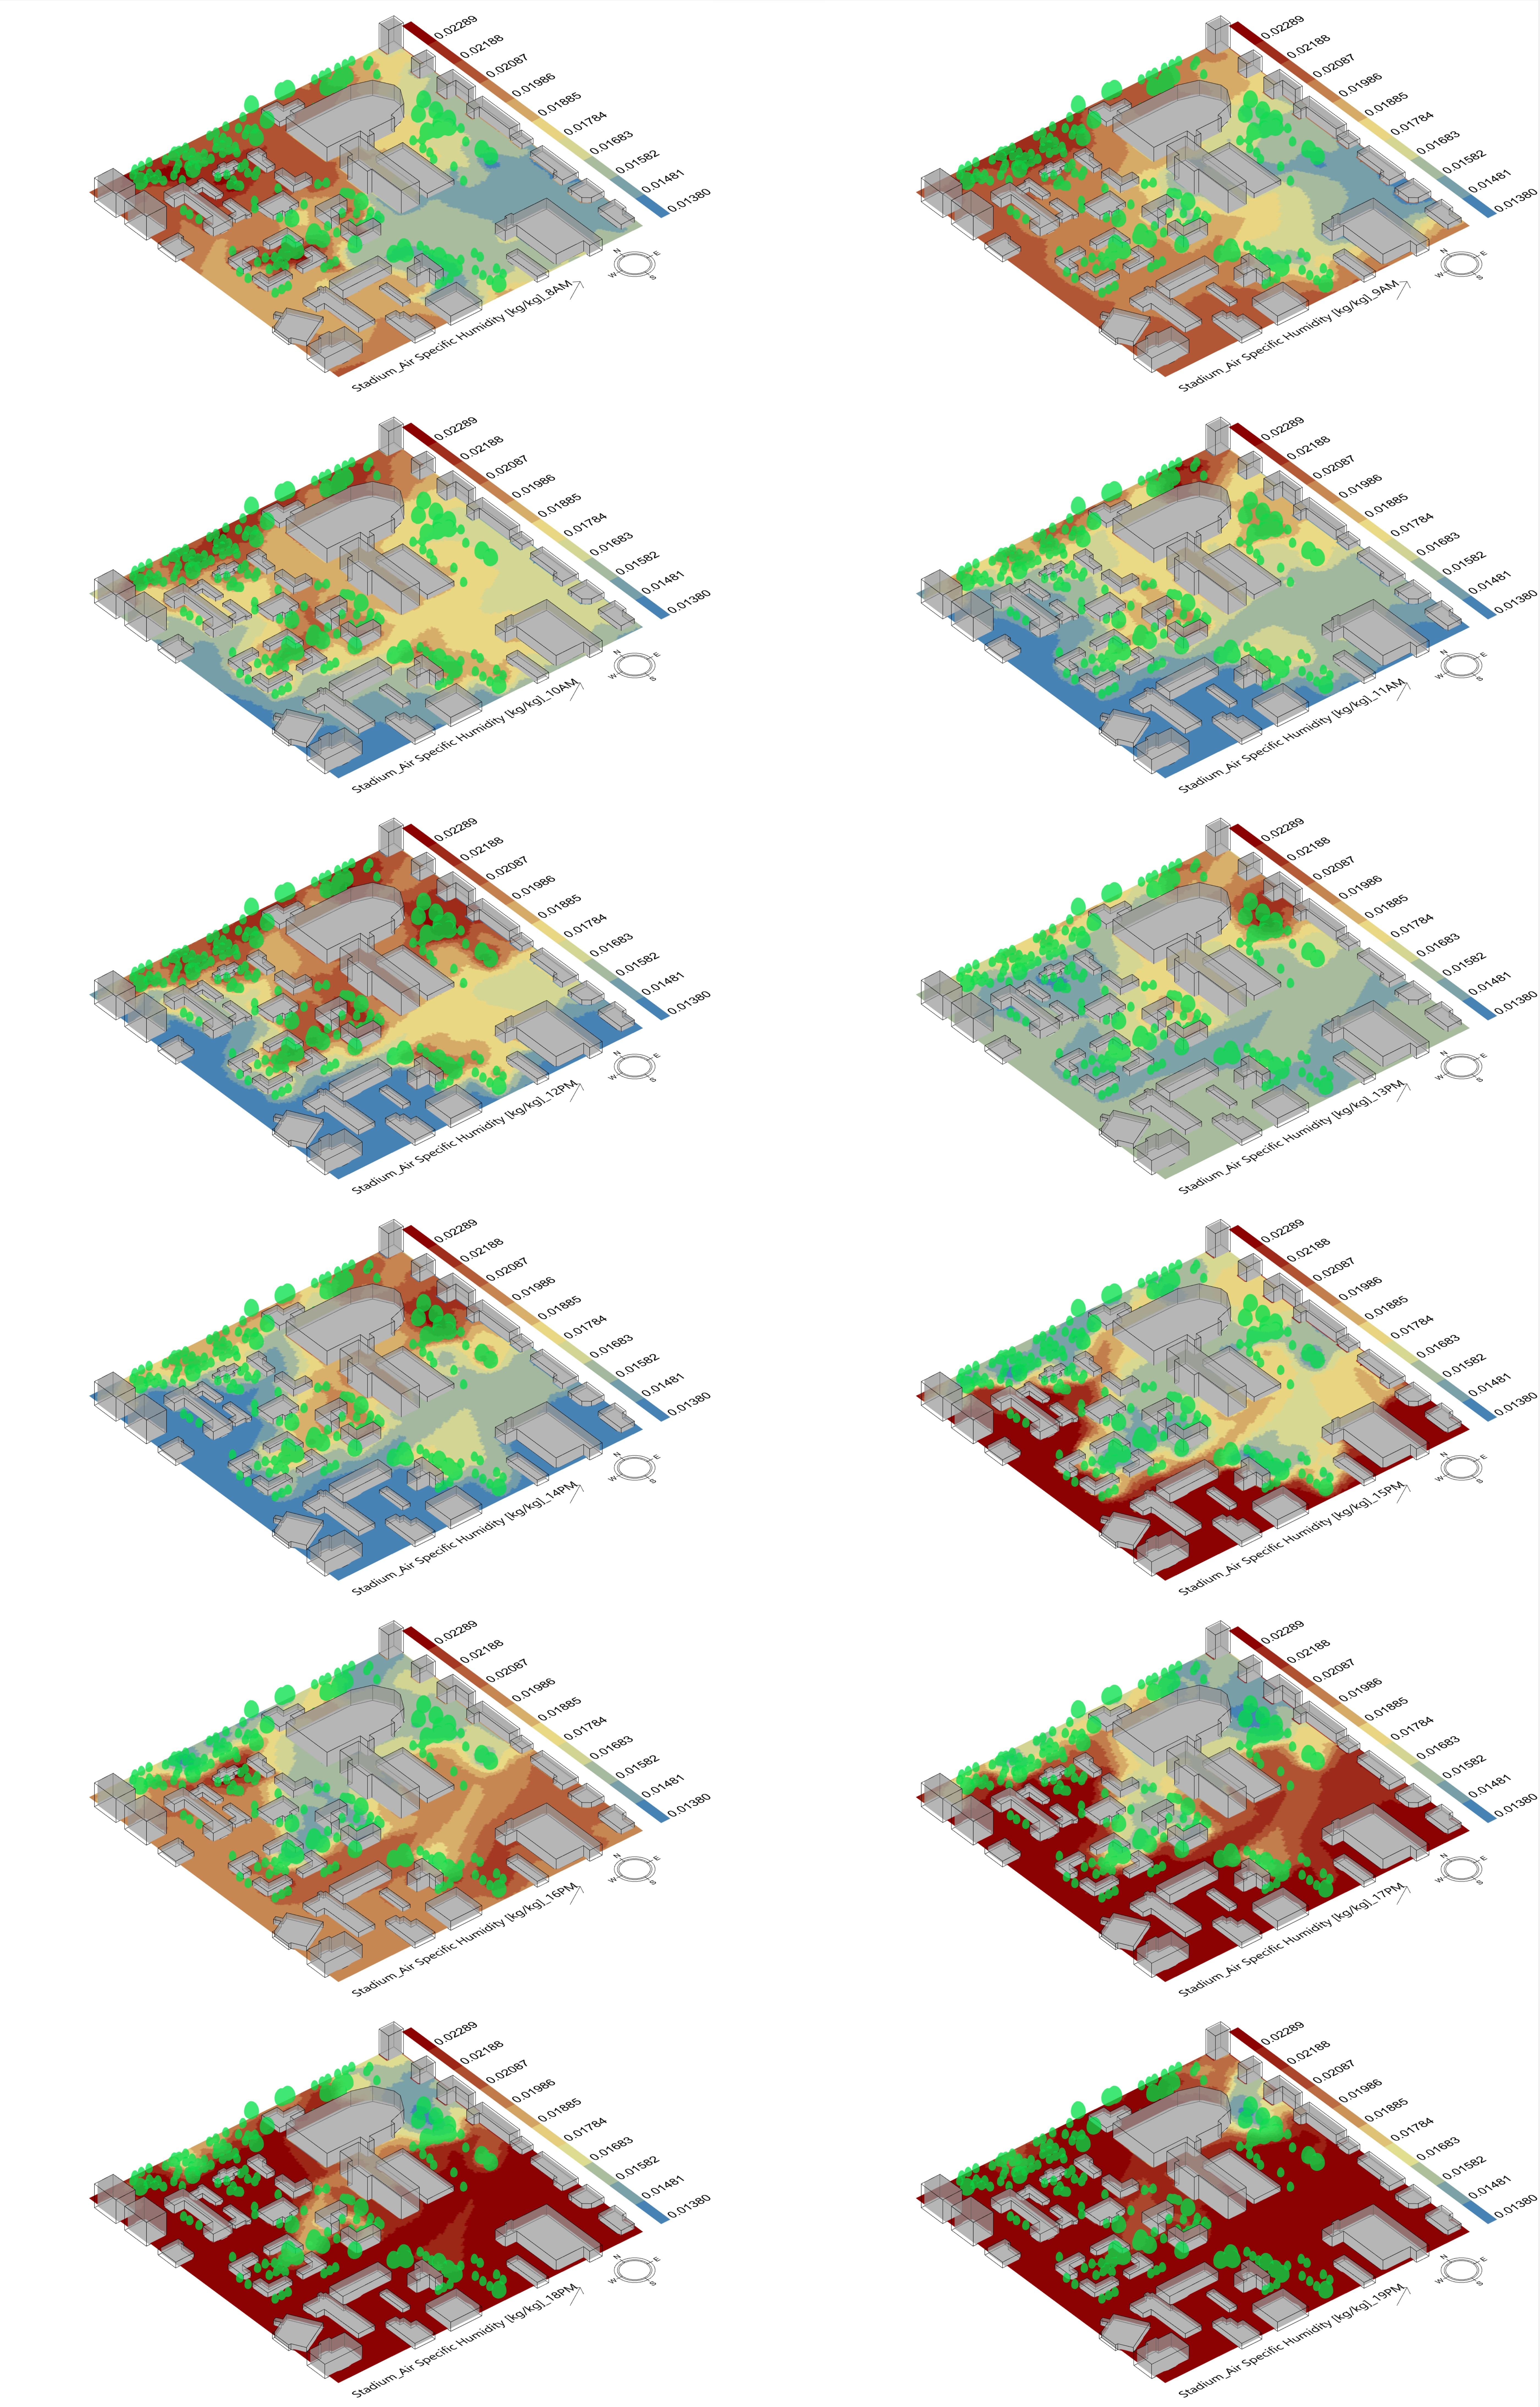
\includegraphics[width=0.9\linewidth]{figures/edcenter_humidity_table.jpg}
    \caption{Educational center specific humidity Outdoor+ simulation results heatmap from 8AM to 7PM.}
    \label{fig:outdoorplus_edcenter_humidity_table}
\end{figure}

%envimet humidity table
\begin{figure}
    \centering
    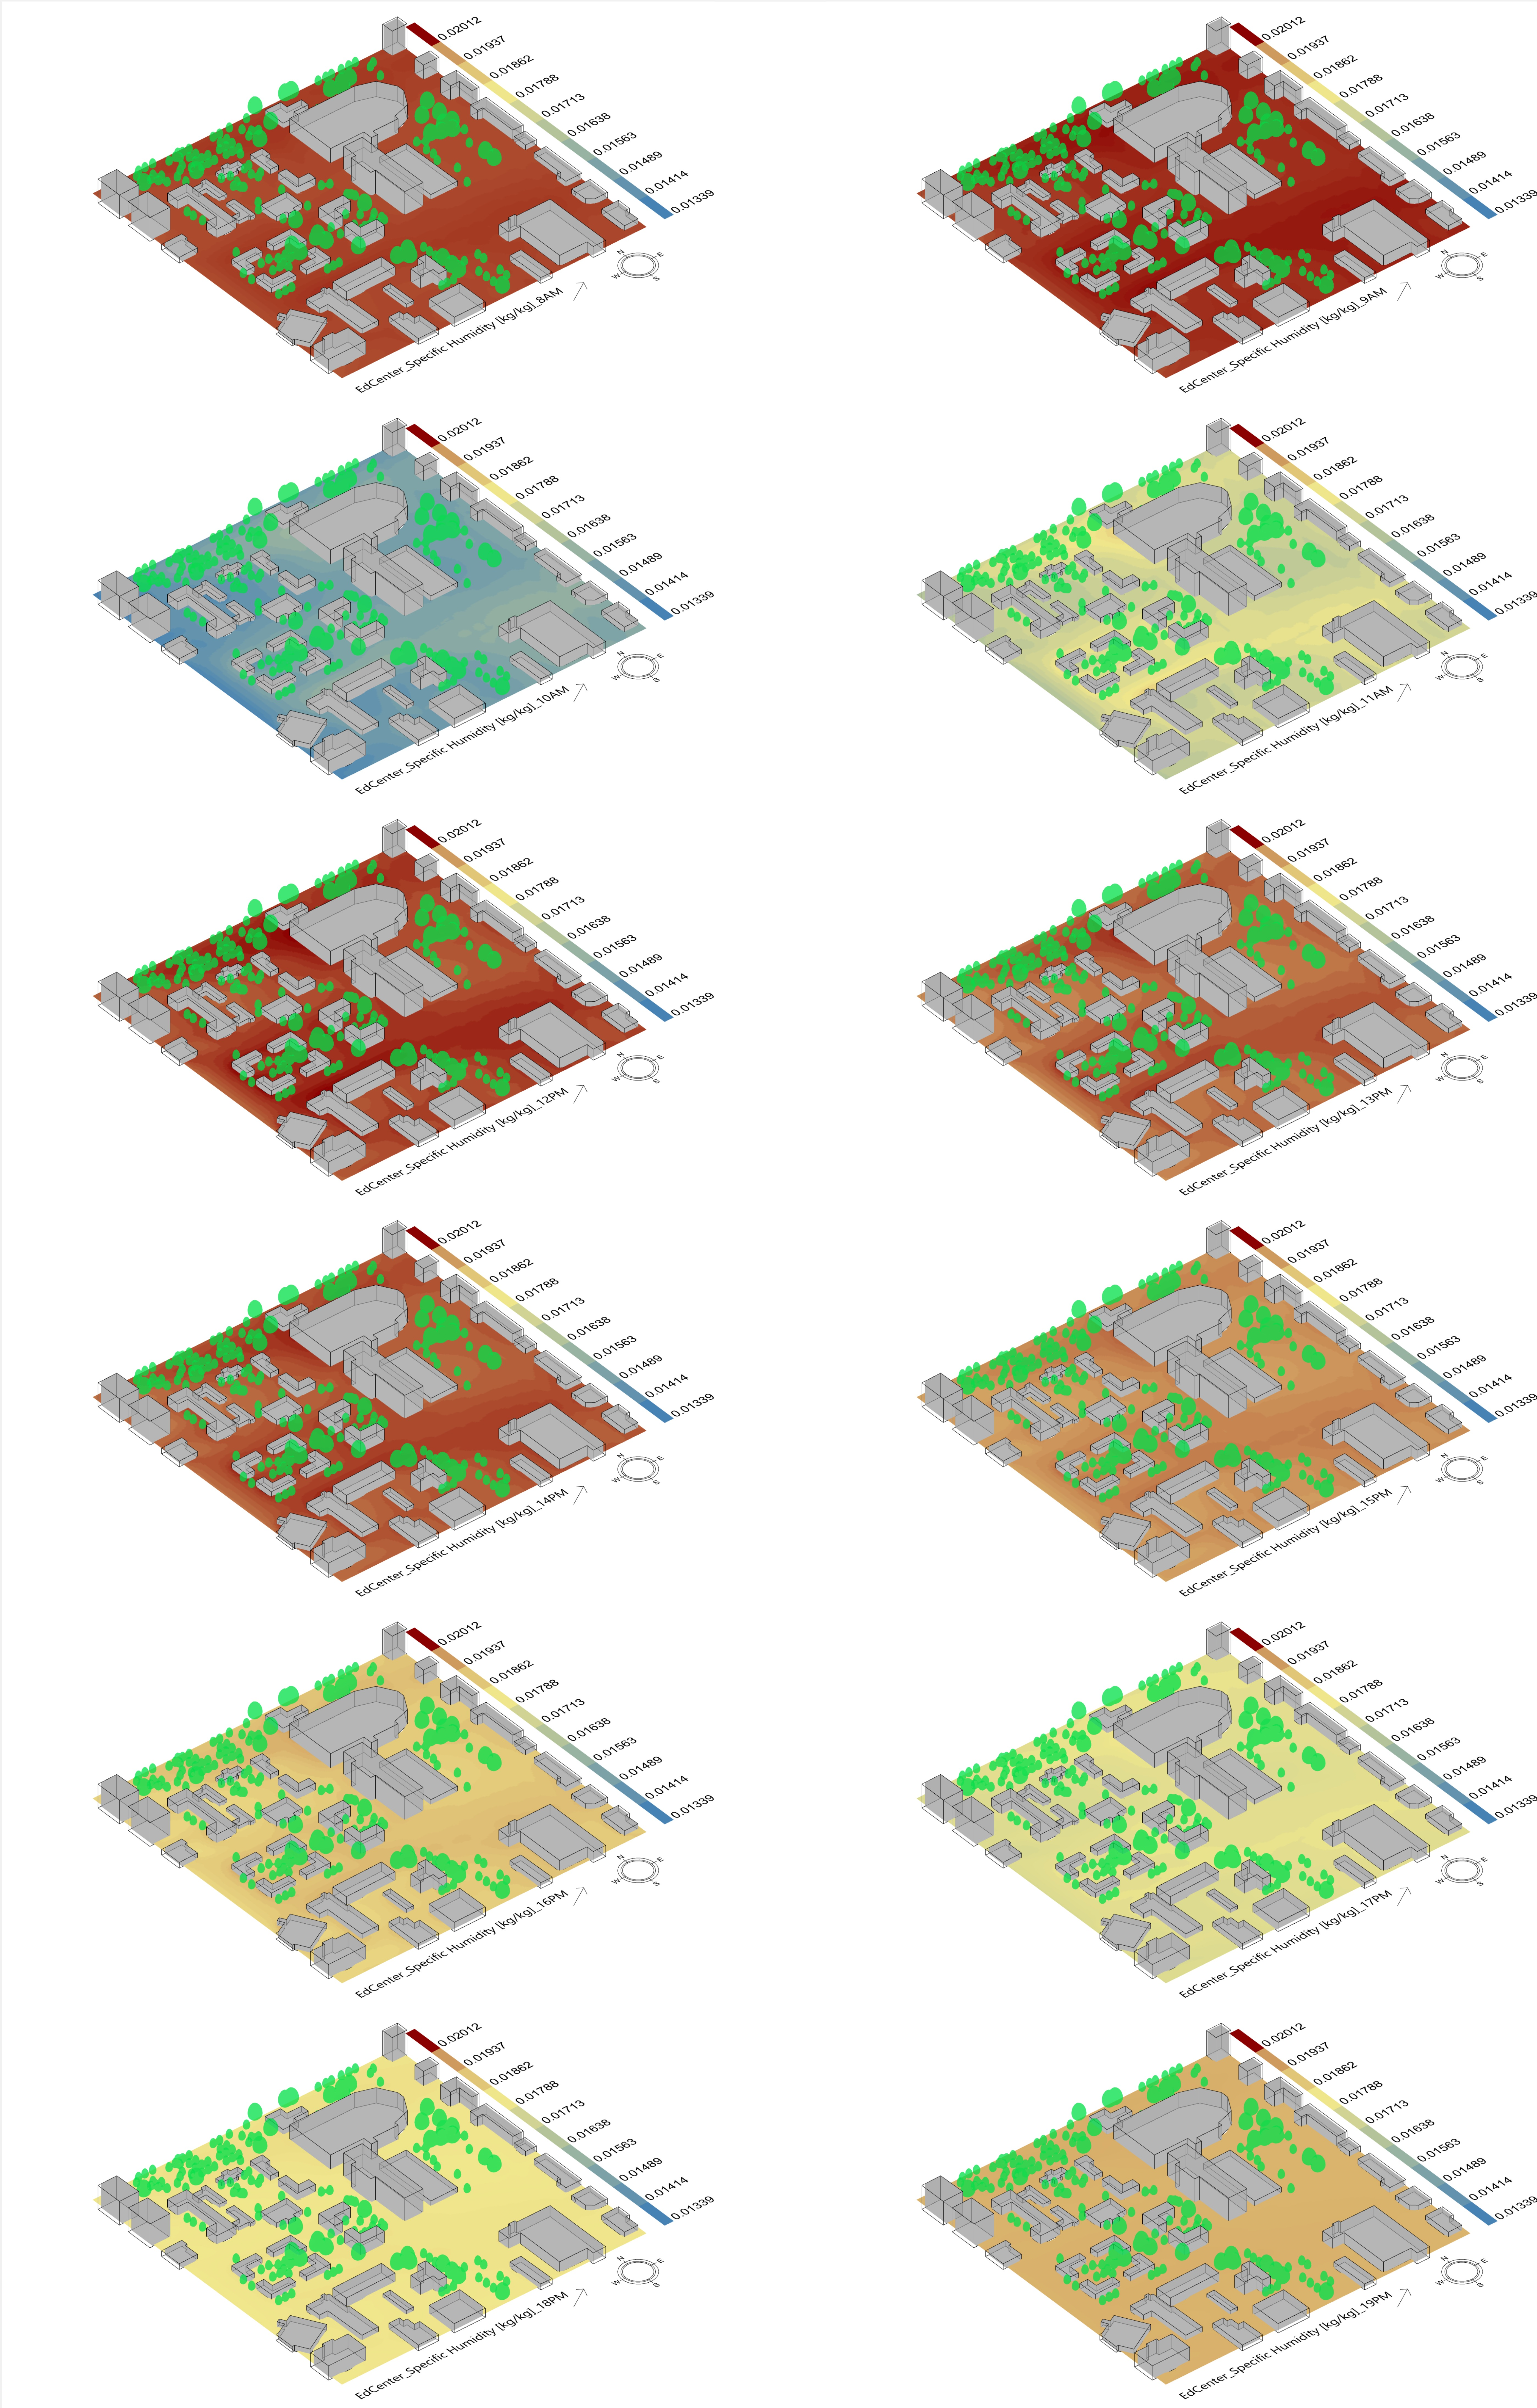
\includegraphics[width=0.9\linewidth]{figures/envimet_edcenter_humidity_table.jpg}
    \caption{Educational center specific humidity ENVI-met simulation results heatmap from 8AM to 7PM.}
    \label{fig:envimet_edcenter_humidity_table}
\end{figure}

\clearpage
\ref{fig:edcenter_humidity_scatterplot} shows the specific humidity results comparing both tools in the scatter plot format. The scatter plot consists of two small clusters in which comparatively high Outdoor+ specific humidity values align with low ENVI-met values. The third large cluster indicates that ENVI-met produces higher specific humidity values ranging from 0.018 kg/kg to 0.020 kg/kg, compared to Outdoor+ ranging from 0.014 kg/kg up to 0.022 kg/kg. For this reduced ENVI-met specific humidity range, Outdoor+ captures more variation with lower values overall. The data points distribution is stretched in the predicted axis, resulting in negligible agreement regarding the 1:1 line.

%edcenter humidity scatterplot
\begin{figure}[H]
    \centering
    \includegraphics[width=0.9\linewidth]{figures/educational_center_-_humidity_scatter_plot_scatter.png}
    \caption{Educational center specific humidity scatter plot: observed (ENVI-met) vs. predicted (Outdoor+}
    \label{fig:edcenter_humidity_scatterplot}
\end{figure}

\clearpage
\ref{fig:edcenter_humidity_timeline_14089}, \ref{fig:edcenter_humidity_timeline_22076}, \ref{fig:edcenter_humidity_timeline_27408}, and \ref{fig:edcenter_humidity_timeline_33635} illustrate the specific humidity values at specific probing points from 8AM to 7PM. The probing points ID 14089, 22076, 27408, and 33635 show the same trend for Outdoor+ results alignment with the boundary reference values. While the boundary reference values are constant and equal for all four probing points, Outdoor+ shows higher values during morning hours, decreasing below the boundary reference values during afternoon hours. On the other hand, ENVI-met values start with lower values, decreasing at 10AM, and reaching the highest specific humidity values around midday. The highest difference percentages range from 44.4\% up to 49.0\%. Values tend to align after 3PM -- 4PM, with difference percentages ranging from 0.5\% to 13.1\%.

%edcenter humidity timeline plots
\begin{figure}[H]
    \centering
    \includegraphics[width=1\linewidth]{figures/educational_center_-_humidity_timeline_14089_timeline.png}
    \caption{Educational center specific humidity timeline plot for point 14089 'exposed'.}
    \label{fig:edcenter_humidity_timeline_14089}
\end{figure}

\begin{figure}[H]
    \centering
    \includegraphics[width=1\linewidth]{figures/educational_center_-_humidity_timeline_22076_timeline.png}
    \caption{Educational center specific humidity timeline plot for point 22076 'covered'.}
    \label{fig:edcenter_humidity_timeline_22076}
\end{figure}

\begin{figure}[H]
    \centering
    \includegraphics[width=1\linewidth]{figures/educational_center_-_humidity_timeline_27408_timeline.png}
    \caption{Educational center specific humidity timeline plot for point 27408 'entrance'.}
    \label{fig:edcenter_humidity_timeline_27408}
\end{figure}

\begin{figure}[H]
    \centering
    \includegraphics[width=1\linewidth]{figures/educational_center_-_humidity_timeline_33635_timeline.png}
    \caption{Educational center specific humidity timeline plot for point 33635 'open area'.}
    \label{fig:edcenter_humidity_timeline_33635}
\end{figure}

The educational center wind speed heatmap results are shown in \ref{fig:outdoorplus_edcenter_windspeed_table} and \ref{fig:envimet_edcenter_windspeed_table}. Outdoor+ wind speed heatmaps expose similar vector magnitude distribution compared to the previous stadium case study results. For some locations, wind speed values vary over time, capturing a wider range. Outdoor+ geometry also influences the wind speed values due to buildings and trees blockage, and buildings corners effect. Differently, ENVI-met wind speed results show a constant, steady wind flow pattern over time. Regardless of the less variation within the simulation domain plane containing the wind speed values, it still captures variations where the wind speed decreases when blocked by buildings or trees.

%outdoorplus wind speed table
\begin{figure}[H]
    \centering
    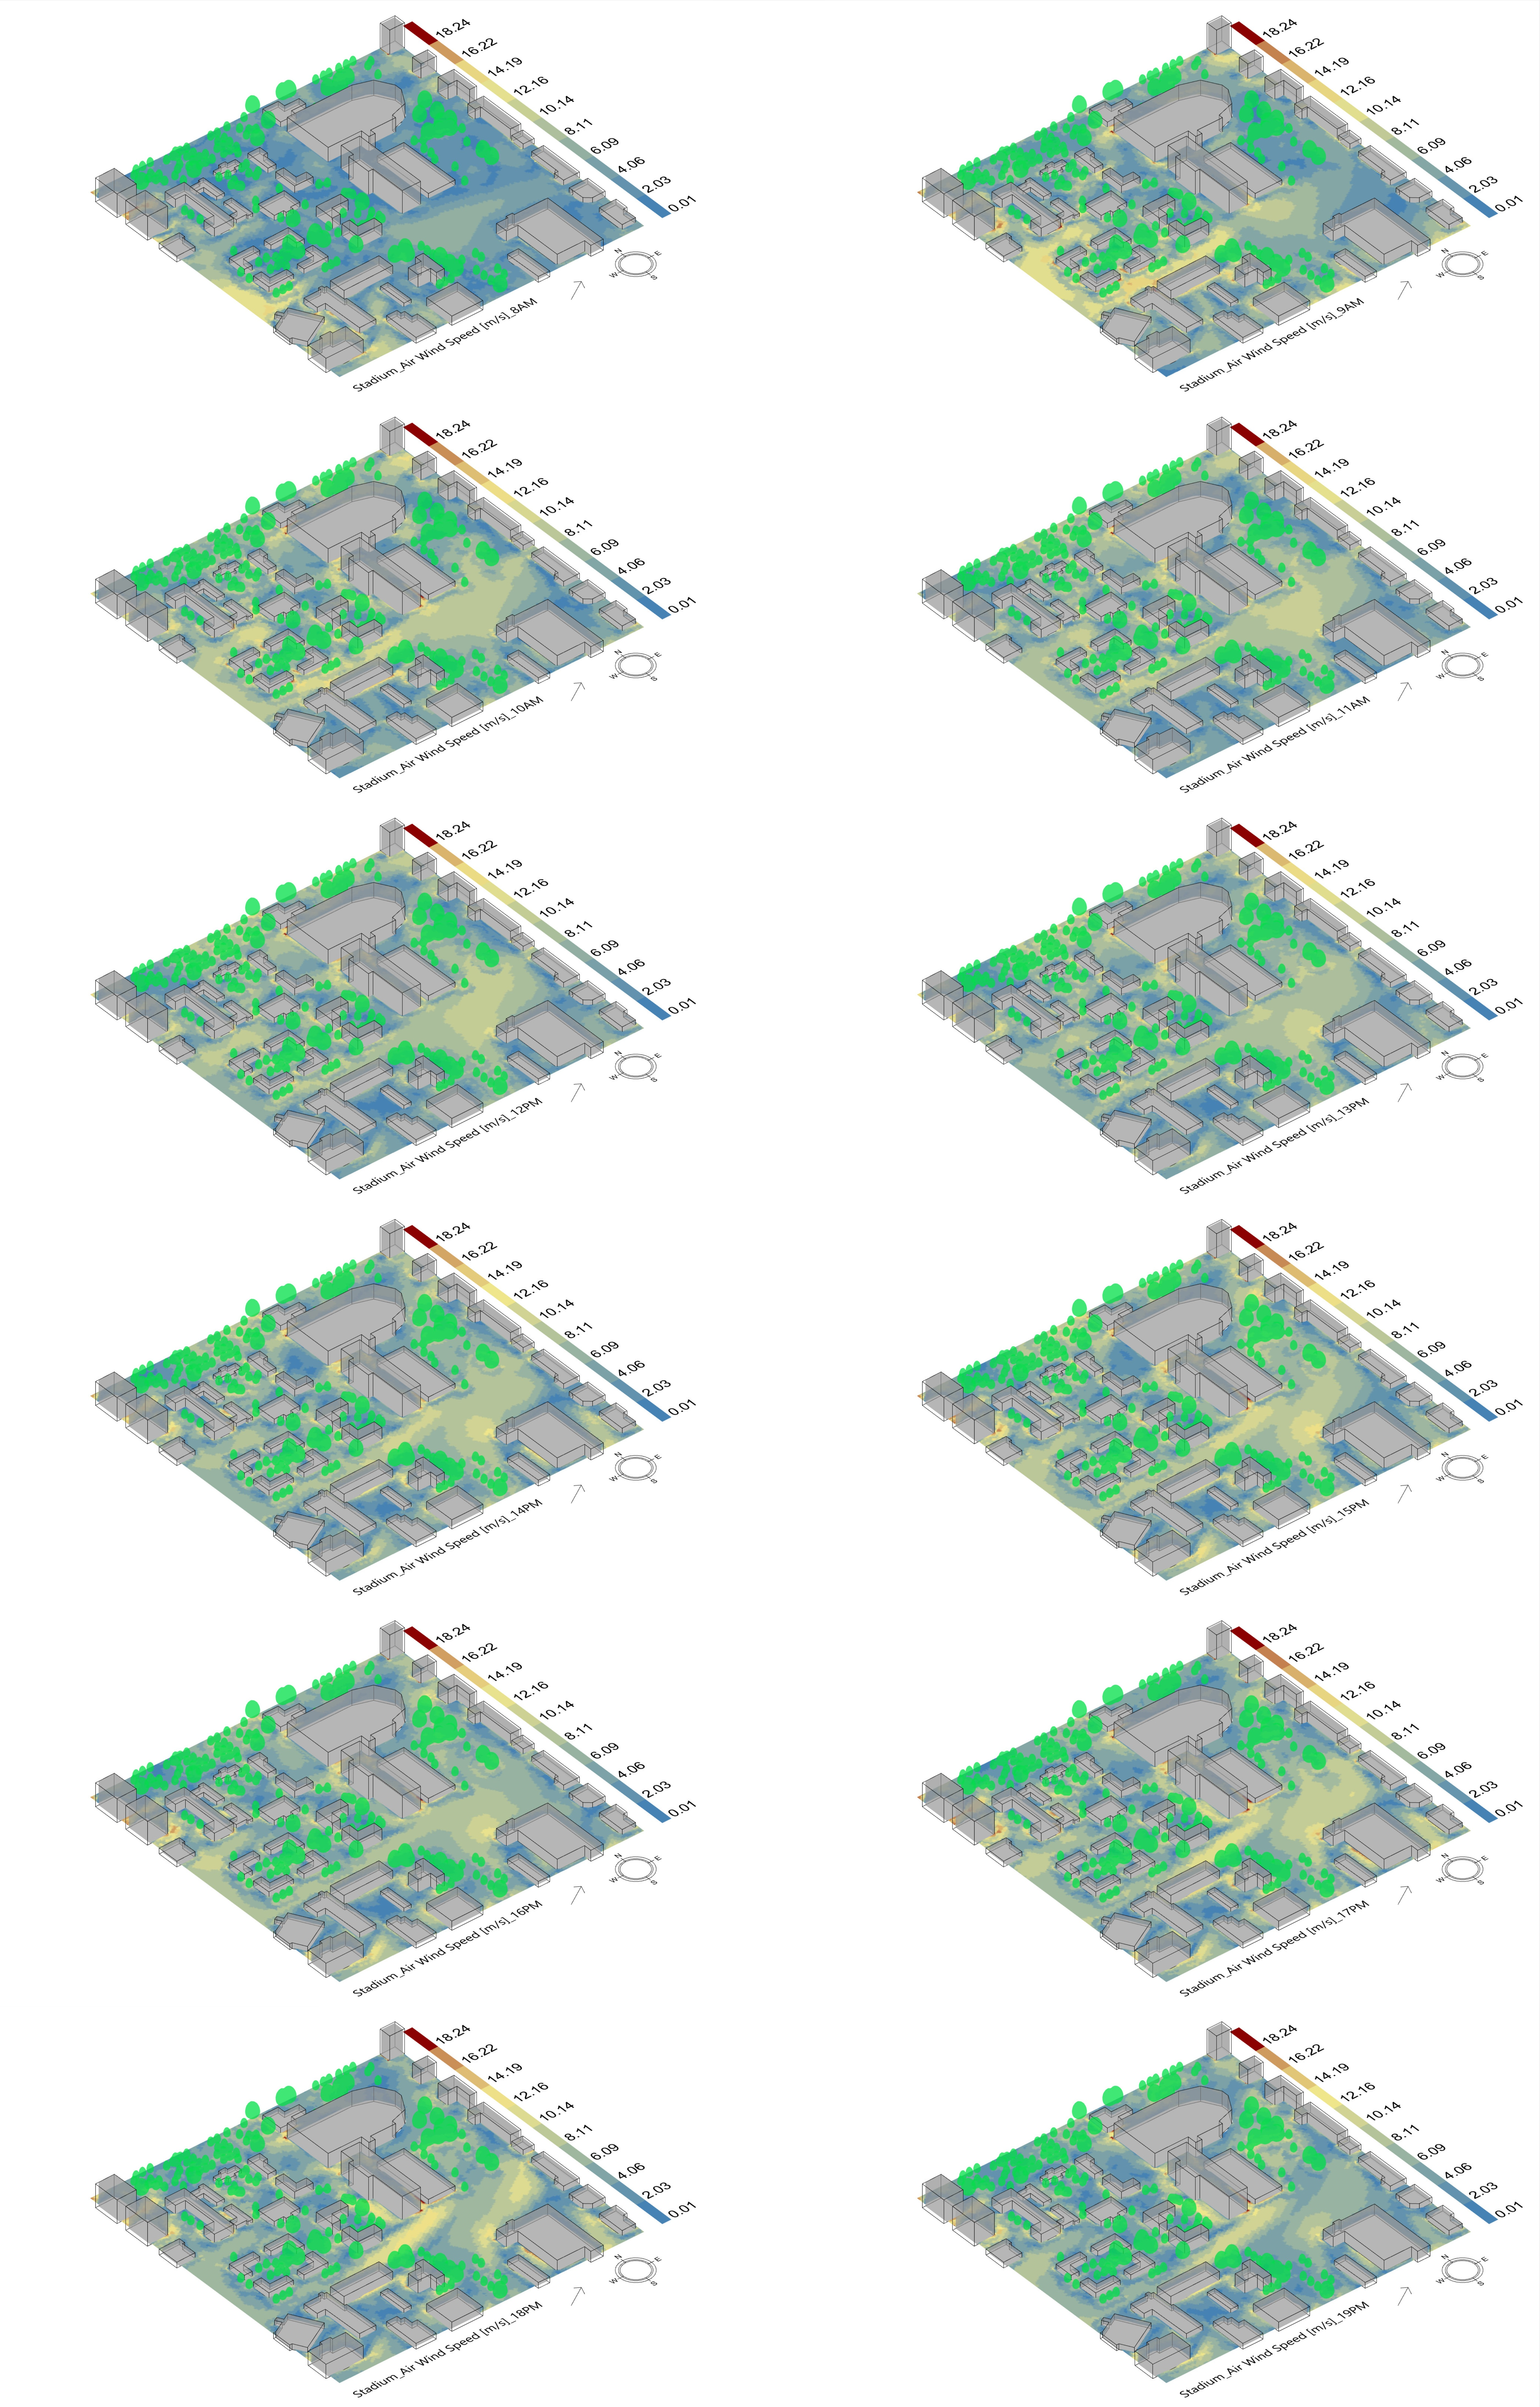
\includegraphics[width=0.9\linewidth]{figures/edcenter_windspeed_table.jpg}
    \caption{Educational center wind speed Outdoor+ simulation results heatmap from 8AM to 7PM.}
    \label{fig:outdoorplus_edcenter_windspeed_table}
\end{figure}

%envimet wind speed table
\begin{figure}[H]
    \centering
    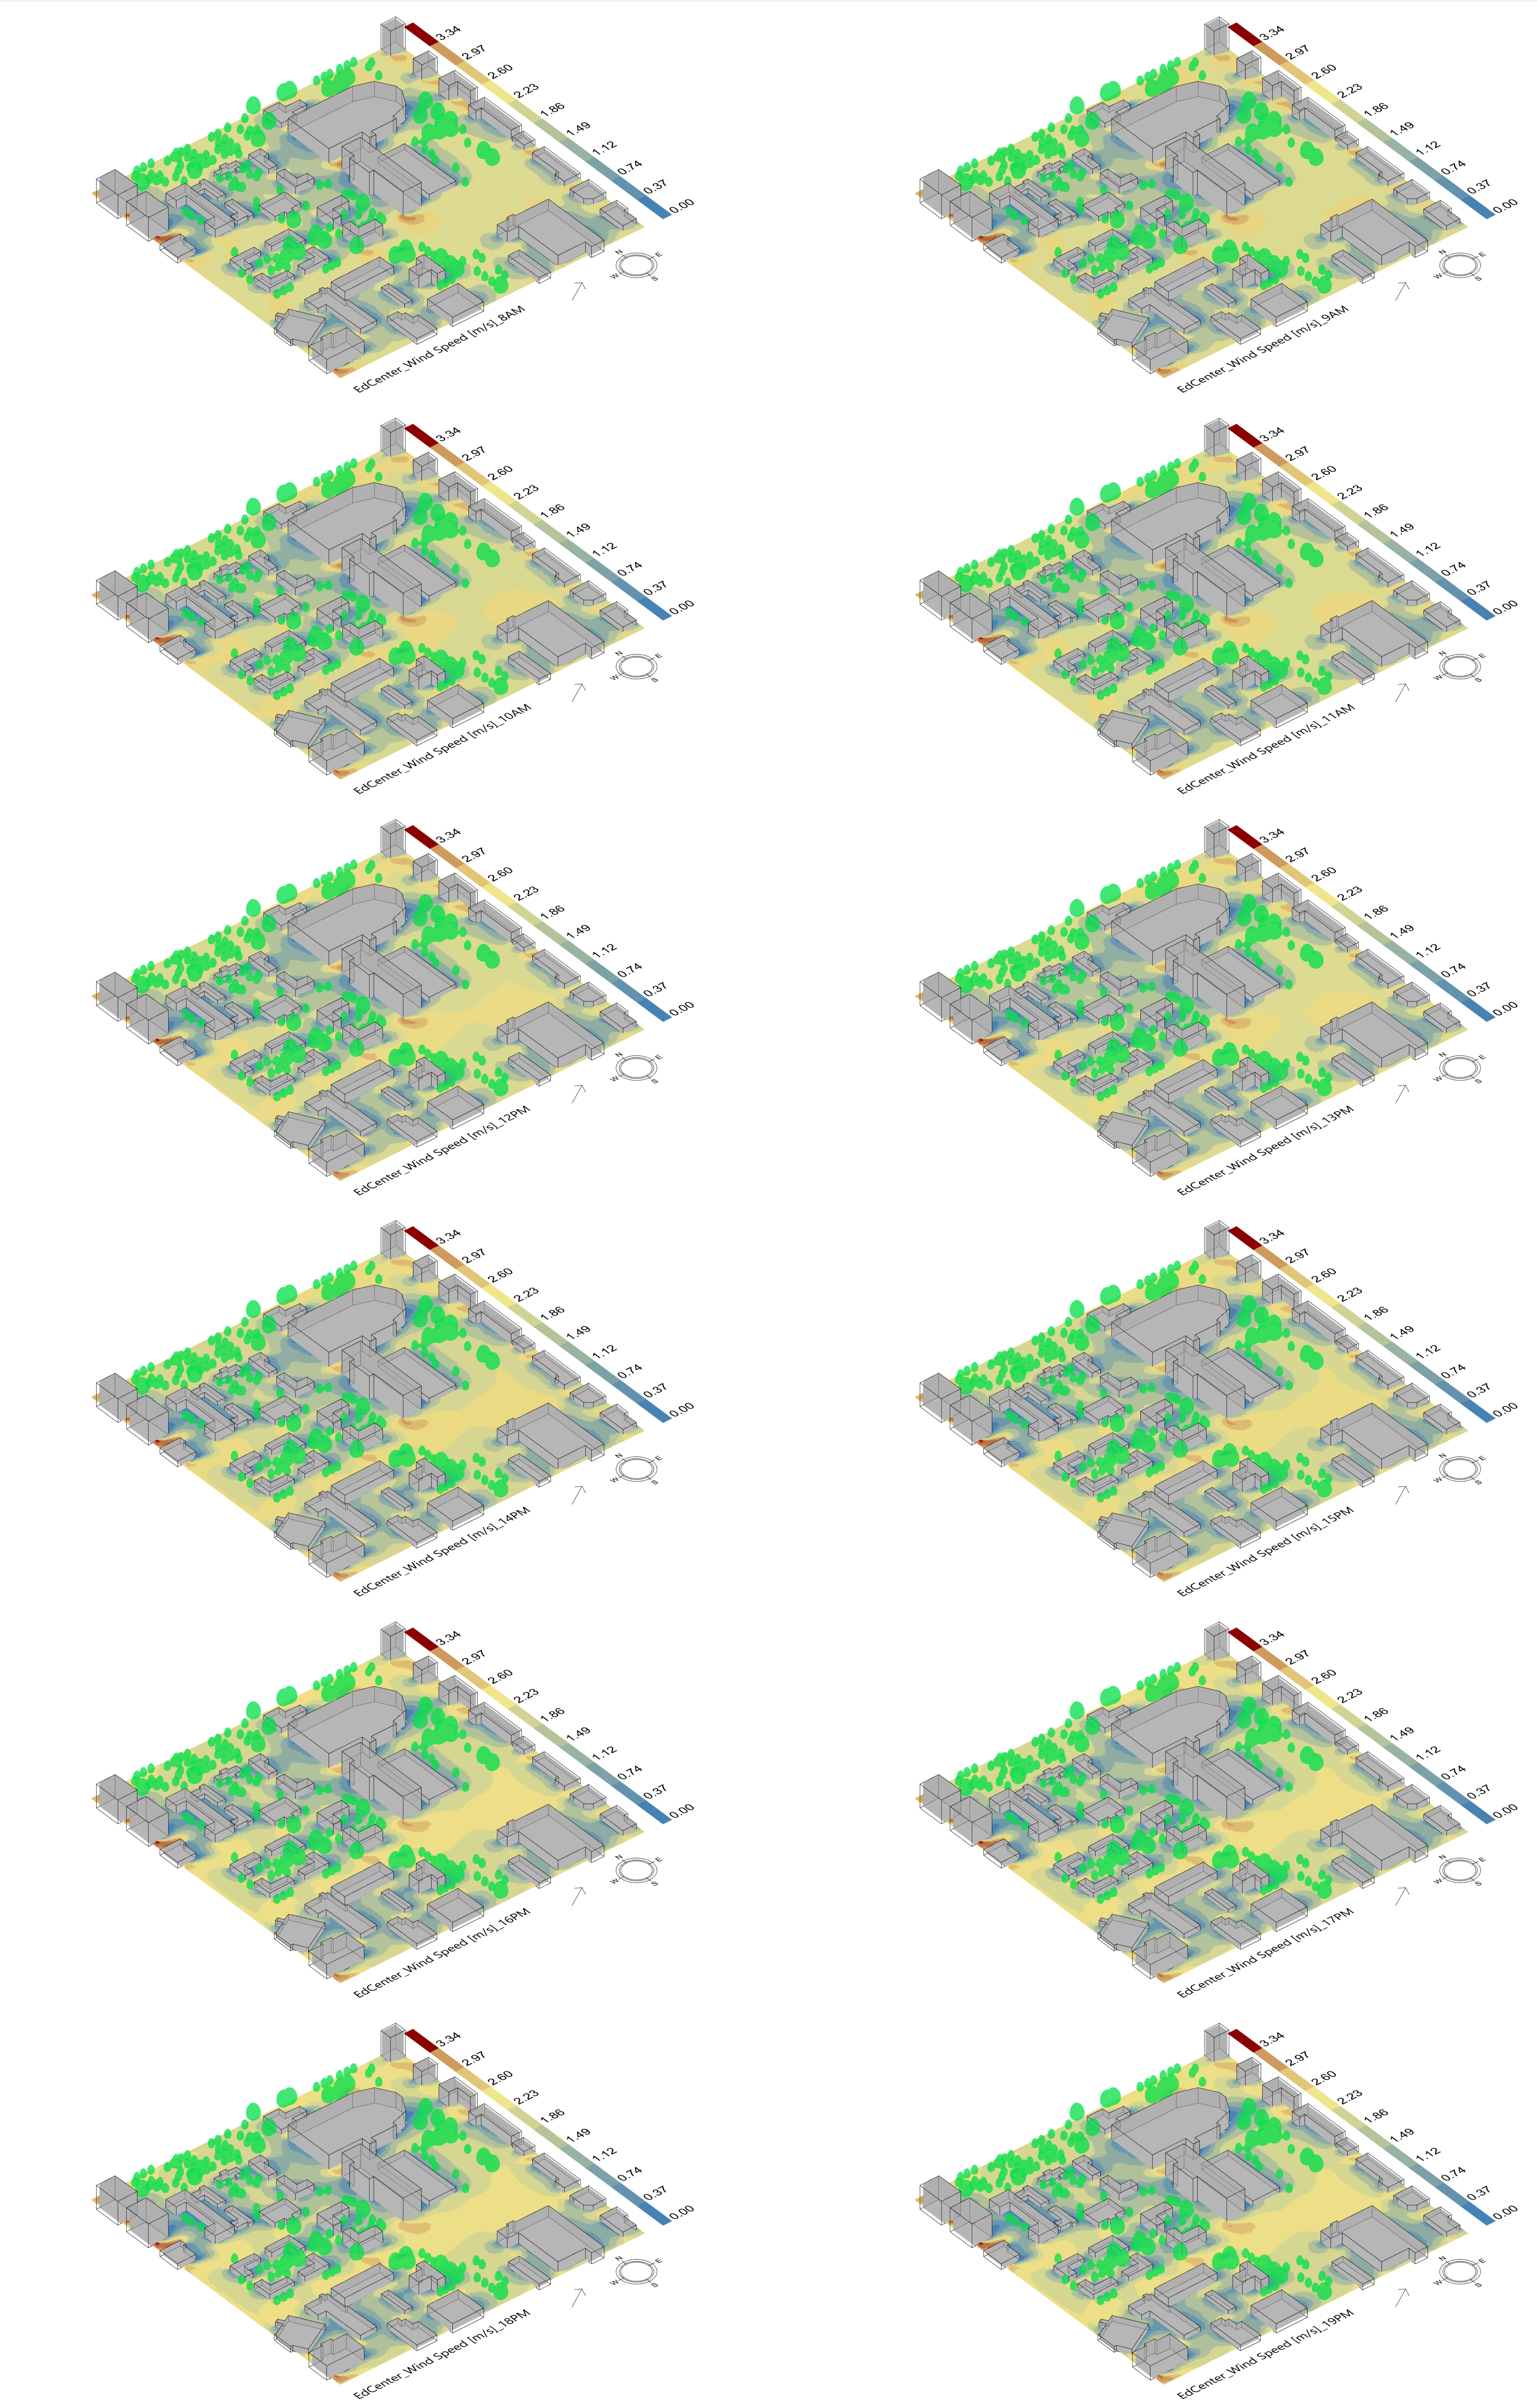
\includegraphics[width=0.9\linewidth]{figures/envimet_edcenter_windspeed_table.jpg}
    \caption{Educational center wind speed ENVI-met simulation results heatmap from 8AM to 7PM.}
    \label{fig:envimet_edcenter_windspeed_table}
\end{figure}

\ref{fig:edcenter_windspeed_scatterplot} shows the wind speed value distribution comparing both observed and predicted values for ENVI-met and Outdoor+, respectively. The largest portion of all values are contained within the range of 0.0 m/s and 2.5 m/s for ENVI-met values, and 0.0 m/s to 5.0 m/s for Outdoor+ values. However, Outdoor+ presents substantially higher wind speed values up to 17.5 m/s, while ENVI-met values do not show the same variation. This dataset distribution pattern is consistent with the previous stadium case study, in which Outdoor+ captures more wind speed variations inside the probing plane within the simulation domain.

%edcenter wind speed scatter plot
\begin{figure}[H]
    \centering
    \includegraphics[width=0.9\linewidth]{figures/educational_center_-_wind_speed_scatter_plot_scatter.png}
    \caption{Educational center wind speed scatter plot: observed (ENVI-met) vs. predicted (Outdoor+}
    \label{fig:edcenter_windspeed_scatterplot}
\end{figure}

\clearpage
The educational center case study wind speed timeline plots are illustrated in \ref{fig:edcenter_windspeed_timeline_14089}, \ref{fig:edcenter_windspeed_timeline_22076}, \ref{fig:edcenter_windspeed_timeline_27408}, and \ref{fig:edcenter_windspeed_timeline_33635}. The four timeline plots follow the same overall pattern, where ENVI-met does not present notable wind speed variations over time, represented by the horizontal line. However, Outdoor+ wind speed values start higher around 2.0 m/s and decreasing to values below 1.0 m/s over time. Due to the contrast of both wind speed values over time, the percentage differences range from 31.6\% to 145.9\% at 8AM, and 37.1\% to 79.8\% at 7PM. These percentage differences scale to high values due to Outdoor+ wind speed values below 1.0 m/s.

%edcenter wind speed timeline plots
\begin{figure}[H]
    \centering
    \includegraphics[width=1\linewidth]{figures/educational_center_-_wind_speed_timeline_14089_timeline.png}
    \caption{Educational center wind speed timeline plot for point 14089 'exposed'.}
    \label{fig:edcenter_windspeed_timeline_14089}
\end{figure}

\begin{figure}[H]
    \centering
    \includegraphics[width=1\linewidth]{figures/educational_center_-_wind_speed_timeline_22076_timeline.png}
    \caption{Educational center wind speed timeline plot for point 22076 'covered'.}
    \label{fig:edcenter_windspeed_timeline_22076}
\end{figure}

\begin{figure}[H]
    \centering
    \includegraphics[width=1\linewidth]{figures/educational_center_-_wind_speed_timeline_27408_timeline.png}
    \caption{Educational center wind speed timeline plot for point 27408 'entrance'.}
    \label{fig:edcenter_windspeed_timeline_27408}
\end{figure}

\begin{figure}[H]
    \centering
    \includegraphics[width=1\linewidth]{figures/educational_center_-_wind_speed_timeline_33635_timeline.png}
    \caption{Educational center wind speed timeline plot for point 33635 'open area'.}
    \label{fig:edcenter_windspeed_timeline_33635}
\end{figure}